\documentclass[../main.tex]{subfiles}
\graphicspath{{\subfix{../images/}}}
\begin{document}
\section*{Term 2 Week 6}
\begin{enumerate}
    \item 
    We know that the side length of each square is 4.\\
    Consider the three points indicated in the diagram. If we position the circle on axes so that one point is at the origin, we can work out the coordinates of the other two points.
    \begin{figure}[H]
        \centering
        \begin{subfigure}{0.4\textwidth}
            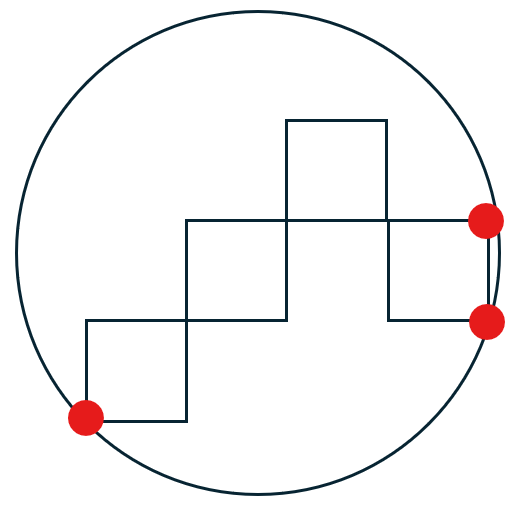
\includegraphics[width=0.5\linewidth]{images/t2w6q1_2.png}
        \end{subfigure}
        \begin{subfigure}{0.4\textwidth}
            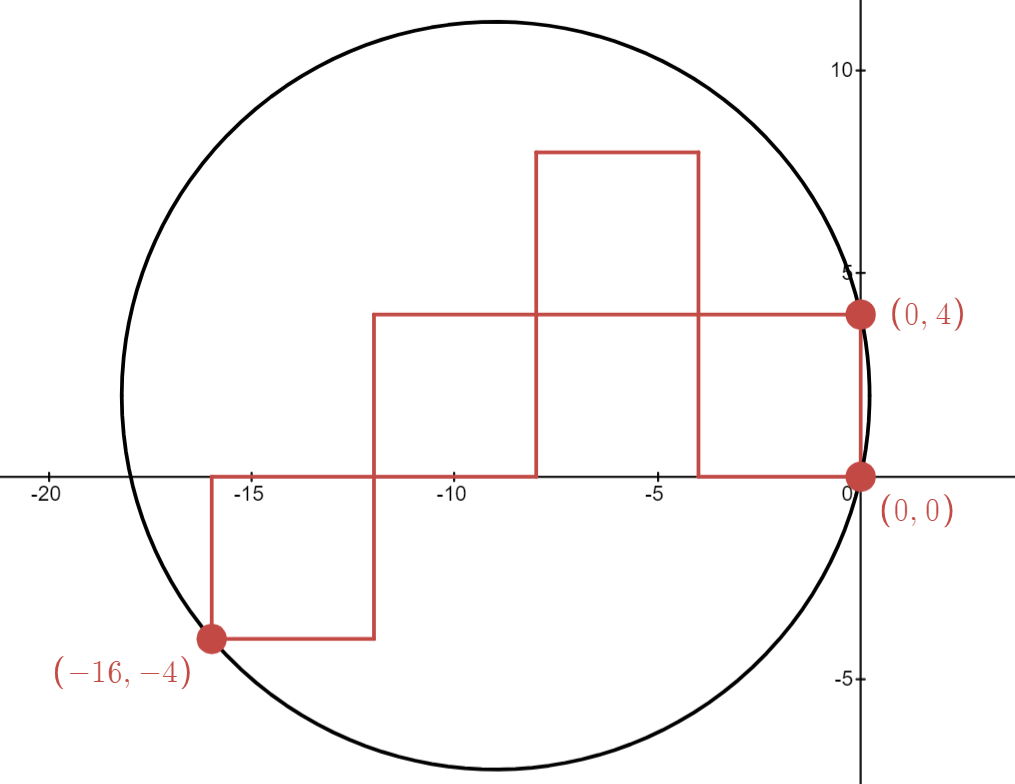
\includegraphics[width=0.7\linewidth]{images/t2w6q1_3.png}
        \end{subfigure}
    \end{figure}
    
    We know the general equation for a circle is \((x-a)^2+(y-b)^2=r^2\), so we can now substitute in the three points to find the equation.\\

    \(0-a)^2+(0-b)^2=r^2\)\\
    \(a^2+b^2=r^2\)\\

    \(0-a)^2+(4-b)^2=r^2\)\\
    \(a^2+16-8b+b^2=r^2\)\\

    \((-16-a)^2+(-4-b)^2=r^2\)\\
    \(256+32a+a^2+16+8b+b^2=r^2\)\\
    \(a^2+32a+b^2+8b+272=r^2\)\\

    Combining equations 1 and 2 by equating the right-hand sides:\\
    \(a^2+16-8b+b^2=a^2+b^2\)\\
    \(16-8b=0\)\\
    \(b=2\)\\

    So our model now looks like this: \((x-a)^2+(b+2)^2=r^2\)\\

    Substituting this into equations 1 and 3, we get:\\
    \(a^2+4=r^2\)\\
    
    \(a^2+32a+4+16+272=r^2\)\\
    \(a^2+32a+292=r^2\)\\
    
    Combining these two by subtracting 1 from 2:\\
    \(32a+288=0\)\\
    \(a=-9\)\\
    
    So our model now looks like \((x+9)^2+(b-2)^2=r^2\)\\

    Substituting in the point (0,0), we get:\\
    \((-9)^2+(2)^2=r^2\)\\
    \(r^2=85\)\\

    We use this and substitute into the area formula:\\
    \(A=\pi r^2\)\\
    \(A=85\pi\)\\
    
    \item 
    If \(a^2+b^2+c^2+d^2=4\):
    Where \(a,b,c,d \in \mathbb{R}\):
        \begin{enumerate}
            \item 
            Show that \((a+2)(b+2)\geq cd\)\\
            Expanding:\\
            \(ab+2a+2b+4\geq cd\)\\
            \(ab-cd+2a+2b+4\geq 0\)\\
            Doubling to get 2ab and -2cd, which are terms we would get if we expanded \((a+b)^2\) and \((c-d)^2\):\\
            \(2ab-2cd+4a+4b+8\geq 0\)\\

            We can substitute the \(a^2+b^2+c^2+d^2\) for 4:\\
            \(a^2+b^2+c^2+d^2+2ab-2cd+4a+4b+4 \geq 0\)\\

            Now if we factorise:\\
            \((a+b)^2+(c-d)^2+4a+4b+4 \geq0\)\\

            Next, consider the expression \((a+b+2)^2\)\\
            Which can be expanded and simplified as follows:\\
            \(a^2+ab+2a+ab+b^2+2b+2a+2b+4=a^2+2ab+b^2+4a+4b+4=(a+b)^2+4a+4b+4\)\\

            This means that \((a+b)^2+(c-d)^2+4a+4b+4 \geq0\)\\ can be rewritten as:\\
            \((a+b+2)^2+(c-d)^2 \geq0\)\\
            
            \item 
            Determine when \((a+2)(b+2)=cd\)\\
            From part (a), this is equivalent to \((a+2)(b+2)=cd\).\\
            Since both \((a+b+2)^2\) and \((c-d)^2\) will always be non-negative, it means that they must both equal zero.\\
            Therefore, the conditions that hold are \(a+b=-2\) and \(c=d\).
        \end{enumerate}

    \item 
    \(\log_{\log_3{x}}{9}=\log_3{(\log_{27}{x})}\)\\

    Change to a log base 3:\\

    \(\frac{\log_3 9}{\log_3 (\log_3 x)}=\log_3{(\frac{\log_3 x}{\log_3 27})}\)\\

    \(\frac{2}{\log_3 (\log_3 x)}=\log_3{(\frac{\log_3 x}{3})}\)\\

    \(\frac{2}{\log_3 (\log_3 x)}=\log_3{(\log_3 x)}-\log_3 (3)\)\\

    \(\frac{2}{\log_3 (\log_3 x)}=\log_3{(\log_3 x)}-1\)\\

    \(2=(\log_3 (\log_3 x))^2-\log_3 (\log_3 x)\)\\

    Substituting \(u=\log_3 (\log_3 x)\), we have a quadratic to solve:\\

    \(2=u^2-u\)\\
    \(u^2-u-2=0\)\\
    \(u=-1, 2\)\\

    Back-substituting to solve for \textit{x}:\\
    \(\log_3 (\log_3 x)=-1\)\\
    \(\log_3 x=\frac{1}{3}\)\\
    \(x=\sqrt[3]{3}\)\\
    \(\log_3 (\log_3 x)=2\)\\
    \(\log_3 x=9\)\\
    \(x=3^9=19683\)\\
    
    \item 
    \(\angle CAB\) consists of two angles, so we can write \(\tan{(\angle CAB)}=\tan{(\alpha + \beta)}=\frac{22}{7}\)\\
    From the diagram, \(\tan{(\alpha)}=\frac{3}{h}\) and \(\tan{(\beta)}=\frac{17}{h}\)\\

    Using the tangent compound angle rule:\\
    \(\tan{(\alpha + \beta)}=\frac{\frac{3}{h}+\frac{17}{h}}{1-\frac{3}{h}.\frac{17}{h}}=\frac{22}{7}\)\\

    Rearranging:\\
    \(\frac{\frac{20}{h}}{1-\frac{51}{h^2}}=\frac{22}{7}\)\\

    \(\frac{\frac{20}{h}}{\frac{h^2-51}{h^2}}=\frac{22}{7}\)\\

    \(\frac{20h^2}{h^3-51h^2}=\frac{22}{7}\)\\

    \(\frac{140}{h}=\frac{22(h^2-51)}{h^2}\)\\

    \(140h=22(h^2-51)\)\\

    \(70h=11h^2-561\)\\

    \(11h^2-70h-561=0\)\\
    \(h=\frac{-51}{11}, 11\)\\

    We can ignore the negative solution as the height must be positive.\\
    Therefore, the area of the triangle is \(\frac{1}{2}(3+17)\times 11=110u^2\).
    \end{enumerate}

\end{document}